\chapter{Application: Strong Edge Colouring}
\label{chap:strong_edge_colouring}

As defined in the \hyperref[sec:intro_strong_edge_coloring]{introduction}
a strong edge colouring of a graph is an edge colouring where two edges which are incident to some
common edge must have different colours.

We can view a strong edge colouring of a graph as a proper vertex colour of $L(G)^2$, the
square of the line graph of $G$ \cite{molloyBoundStrongChromatic1997}.
The line graph $L(G)$ is a graph with a vertex $v_e$ for
each $e\in E(G)$ such that $\{v_e, v_f\} \in E(L(G))$ iff $e$ is incident to $f$ in
$G$. The square of a graph $G^2$ then is a copy of the graph where vertices at distance $\leq 2$
are connected. See figure \ref{fig:lg_example} for an example construction.

\begin{figure}[ht]
    \centering
    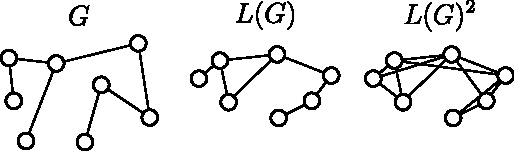
\includegraphics{LG_example}
    \caption{Example $G$, $L(G)$ and $L(G)^2$}
    \label{fig:lg_example}
\end{figure}

\begin{definition}[Strong Neighbourhood]
    Given a graph $G$ and edge $E \in E(G)$ define the strong neighbourhood
    $N_s(e)$ of $e$ as those edges $f \in E(G)$ which are adjacent to $e$ in 
    $L(G)^2$ (i.e. those which cannot share a colour with $e$ in a strong edge colouring).
\end{definition}

\section{The Erd\H{o}s and Nešetřil conjecture}

Erd\H{o}s and Nešetřil \cite{faudreeInducedMatchingsBipartite1989} conjectured an
upper bound on the strong chromatic index $\chi'_s(G)$, the minimum colours needed for
a strong edge colouring.

\begin{conjecture}[Erd\H{o}s, Nešetřil 1989 \cite{faudreeInducedMatchingsBipartite1989}]
    $\chi'_s(G) \leq 1.25\Delta(G)^2$ for all graphs $G$.
\end{conjecture}

The bound of $2\Delta(G)^2$ was the best known bound until 1997 when Molloy and Reed
showed the following.
\begin{knowntheorem}[Molloy, Reed 1997 \cite{molloyBoundStrongChromatic1997}]
    $\chi'_s(G) \leq 1.998\Delta(G)^2$ for $\Delta(G)$ sufficiently large.
\end{knowntheorem}

Their proof consisted of colouring $L(G)^2$ with 2 discrete steps:
The first is a bound on the edge density of any neighbourhood of $L(G)^2$. We call
this the \textit{strong neighbourhood density}.
\begin{knownlemma}[Lemma 1 from \cite{molloyBoundStrongChromatic1997}]
    If $G$ has maximum degree $\Delta$ then for each $e\in E(G)$
    $|N_s(e)| \leq (1-\frac{1}{36})\binom{2\Delta^2}{2}$.
\end{knownlemma}
After showing the strong neighbourhoods in $L(G)^2$ are sparse they use a colouring
lemma to colour $L(G)^2$:
\begin{knownlemma}[Lemma 2 from \cite{molloyBoundStrongChromatic1997}]
    Let $\delta, \gamma > 0$ satisfy some condition. Then if
    $\Delta(H) \leq X$ such that $N(v)$ has at most $(1-\delta)\binom{X}{2}$ edges
    then $\chi(H)\leq (1-\gamma)X$.
\end{knownlemma}

This strategy of bounding the edge density of strong neighbourhoods of $G$ and
using a probabilistic colouring was iterated on through successive papers:
Bruhn and Joos found an asymptotically tight bound on the strong neighbourhood density
and improved the colouring lemma.
\begin{knowntheorem}[Bruhn \& Joos, 2015 \cite{bruhnStrongerBoundStrong2018}]
    $\chi'_s(G) \leq 1.93\Delta(G)^2$ for $\Delta(G)$ sufficiently large.
\end{knowntheorem}
Bonamy, Perett and Postle introduced a modification of the method where rather than
bounding the strong edge neighbourhood density for the entire graph we instead focus
on a subgraph of $L(G)^2$ of high degree vertices. They show that the
neighbourhood density in this subgraph can go below the tight bound of Bruhn and Joos
and so can be coloured with fewer colours. The rest of the graph has low degree so can
be coloured greedily.

\begin{knowntheorem}[Bonamy, Perrett \& Postle, 2018 \cite{bonamyColouringGraphsSparse2018}]
    If $\Delta(G)$ is sufficiently large then
    $\chi'_s(G) \leq 1.835\Delta(G)^2$.
\end{knowntheorem}

Most recently then Hurley, de Verclos and Kang improved on the colouring lemma from the
Bonamy et al. paper to achieve the current lowest known bound.
\begin{knowntheorem}[Hurley, de Verclos \& Kang, 2022 \cite{hurleyImprovedProcedureColouring2022}]
    If $\Delta(G)$ is sufficiently large then
    $\chi'_s(G) \leq 1.772\Delta(G)^2$.
\end{knowntheorem}

In this chapter we use the semidefinite method on local flags to improve the strong
neighbourhood density bound, then applying the colouring lemma from Hurley et al. as a black
box we claim the following result.

\begin{theorem}
    \label{thm:strong_edge_colouring_bound}
    If $\Delta(G)$ is sufficiently large then $\chi'_s(G) \leq 1.73\Delta(G)^2$.
\end{theorem}

We will follow the same structure as used in chapter \ref{chap:pentagon_conjecture},
first reducing the problem to a problem on a certain class of coloured graphs,
finding a vector $O$ of local flags for which an asymptotic bound on the density of $O$ will allow
us to derive an asymptotic bound on the size of $E_O(G)$. We then enumerate some elements
of the semantic cone and apply the semidefinite method to get a bound on $O$.

\section{Reduction}

The theorem that we want to improve on is the strong edge neighbourhood theorem from
the Bonamy et al. paper which appears in Hurley et al. as follows:
\begin{knowntheorem}[Theorem 3.1 \cite{hurleyImprovedProcedureColouring2022}]
    Fix $\eta \in [0, 0.3]$. For any graph $G$ let $H=L(G)^2$. Let $F$ be a
    maximum subset of $V(H)$ such that $H[F]$ has minimum degree
    $\geq (2-\eta)\Delta(G)^2$. Then for any $f\in F$ the number of edges in the subgraph
    $H[N_{H[F]}(f)]$ induced by the neighbourhood of $f$ (in $H[F]$) is at most
    \[
        \left(\frac{31}{6} - \frac{128}{10-3\eta} - \eta^2\right)\Delta(G)^4
    \]
\end{knowntheorem}

In other words we are given a graph $G$ and a maximal subset of the edges $F \subseteq E(G)$
such that the subgraph induced by $F$ in $H=L(G)^2$ has minimum degree
$\geq (2-\eta)\Delta(G)^2$ for some $\eta$. This means each $f \in F$ has
at least $(2-\eta)\Delta(G)^2$ other edges $f' \in F$ adjacent in $L(G)^2$
($|N_s(f) \cap F| \geq (2-\eta)\Delta(G)^2\ \forall\ f \in F$).
We can then just consider the graph $H[F]$ induced by this high degree $F$ subset.
Then for some fixed $f \in F$ we want to find an upper bound on the number of edges
in its neighbourhood in $H[F]$. That is, the number of pairs $e, e' \in N_s(f) \cap F$ such
that $e, e'$ adjacent in $L(G)^2$.

\begin{note}
    The first reduction we can note is that WLOG we can assume $G$ is regular,
    as outlined in each of the above papers.
\end{note}

As we did in section \ref{sec:counting_pentagons} we want to reduce this to a problem
on coloured graphs.
Given $G$, $F\subseteq E(H)$, $\eta > 0$ and $f \in F$ as above we can construct a
new corresponding $(2,2)$-graph (red/black vertices, red/black edges) $G'$ as follows:
Let $f=\{u, v\}$. Take a copy of $G$ and colour all neighbours of $u$ and $v$ black
and all other vertices red. Then colour every edge $e \in F$ black and all other
edges red.

\begin{lemma}
    Let $G, F, \eta, f$ and $G'$ be as above.
    Define $E_O(G') \subseteq \binom{E(G')}{2}$ as the set of pairs of edges $e, e'$ in $G'$
    where $e, e'$ are black edges with a common incident edge and
    at least one of the vertices of each edge is black.
    Then the number of edges in $H[N_{H[F]}(f)]$
    where $H=L(G)^2$ is equal to $|E_O(G')| + o(\Delta(G)^4)$.
\end{lemma}

\begin{proof}
    Let $G, F, \eta, f$ and $G'$ be as above. Consider some edge $\{e, e'\}$ in
    $H[N_{H[F]}(f)]$. Both of these $e,e'$ are in $F$ so is coloured black in $G'$.
    Similarly both are in the strong neighbourhood of $F$ meaning each has a common
    incident edge with $f$. Edges incident to $f$ have both vertices coloured black
    in $G'$ so each of $e, e'$ has at least one black vertex.
    Hence this edge $\{e, e'\}$ corresponds to a pair of black edges with at least one
    black vertex each in $G'$ at distance $\leq 2$ from each other.

    Consider then some pair $e,e' \in E_O(G')$
    As each $e,e'$ has a black vertex they must be either incident to $f$ \textit{or} equal
    to $f$. If both $e, e' \neq f$ then
    $e, e'$ satisfy exactly the conditions to be an edge in $H[N_{H[F]}(f)]$.
    Hence we overcount the number of edges in $H[N_{H[F]}(f)]$ by exactly the
    number of these pairs $e, e'\in E_0$ where one of $e, e' = f$. Assume $e=f$,
    this leaves only $\leq 2\Delta(G)^2$ choices for $e'$ so there are at most
    $2\Delta(G)^2$ such pairs which is $o(\Delta(G)^4)$ as required.
\end{proof}

\begin{corollary}
    \label{corollary:strong_density_graph_class}
    It suffices to bound the size of $E_0$
    over the class of all regular $(2,2)$-graphs where there are $\leq 2\Delta(G)^2$ black
    vertices and the subgraph of $L(G)^2$ induced by black edges has minimum
    degree $\geq (2-\eta)\Delta(G)^2$.
\end{corollary}

This is something we can bound with local flags.

\section{Local Flag Setup}

Let $\Gcl$ be the class of graphs described in Corollary \ref{corollary:strong_density_graph_class}.

\begin{lemma}
    Given the class $\Gcl$ and $\Delta$ as the max-degree function then a
    $\sigma$-flag $(F, \theta)\in \HeredG{}^\sigma$ is a local-$\sigma$ flag (definition
    \ref{def:local_flag}) iff
    each connected component of $F$ contains at least one black vertex or labelled vertex.
\end{lemma}

\begin{proof}
    See proof of lemma \ref{lemma:pentagon_local_flags}.
\end{proof}

\subsection{Objective Vector}

First we want to express the size of $E_O(G)$ as a local flag vector.
Note if $\Bcl\subseteq G$ is the set of black edges with at least one black vertex then
\[
    2|E_O(G)| = \sum_{e \in \Bcl}|\{e' \in \Bcl \colon e, e'\ \text{have common edge}\}|
\]
We can split $\Bcl$ further into $\Bcl_1$ and $\Bcl_2$, the set of edges with one
black and one red vertex and the set of edges with two black vertices respectively.
\begin{multline*}
    2|E_O(G)| = \sum_{e \in \Bcl_1}|\{e' \in \Bcl \colon e, e'\ \text{have common edge}\}|\\
    +  \sum_{e \in \Bcl_2}|\{e' \in \Bcl \colon e, e'\ \text{have common edge}\}|
\end{multline*}

The $\sigma_1=\bredge$ is a local type by lemma \ref{lemma:local_type_equiv}. Clearly
for any $e\in \Bcl_1$ we can view $G$ as a $\sigma_1$-flag where $\sigma_1$ is mapped
to $e$. Call this $G^e$. Similarly any $\sigma_1$-embedding corresponds to precisely one
$e\in \Bcl_1$.
Fix some $e\in \Bcl_1$, then take some $e'\in\Bcl$ such that $e,e'$ have a common incident edge.
Then the vertices of $e,e'$ in $G^e$ induce some subgraph of size 4 where the two unlabelled
vertices (those corresponding to $e'$) have a black edge and there is a single connected
component. Conversely any such induced subgraph corresponds to exactly one $e' \in \Bcl$.
Hence we can count such $e'$'s there are by counting how many such induced subgraphs
there are. These subgraphs are easily enumerated.

Define $D(\bredge) \in \Lcl^{\sigma_1}$ to be the vector consisting of the sum of all
local $\sigma_1$-flags of size 4 with a black edge between the unlabelled vertices and a
single connected component:

TODO THIS IS MISSING POSSIBLE BLACK-BLACK RED EDGES IN THE MIDDLE NEEDS REGENERATION.
\[
    \begin{split}
    D(\bredge) &:= 
        \secdbr{4in4t2id2} + \secdbr{5in4t2id2} + \secdbr{6in4t2id2} + \secdbr{10in4t2id2} + \secdbr{13in4t2id2} + \secdbr{14in4t2id2} + \secdbr{15in4t2id2} + \secdbr{19in4t2id2} + \secdbr{20in4t2id2}\\
    &+ \secdbr{21in4t2id2} + \secdbr{25in4t2id2} + \secdbr{28in4t2id2} + \secdbr{29in4t2id2} + \secdbr{31in4t2id2} + \secdbr{32in4t2id2} + \secdbr{39in4t2id2} + \secdbr{40in4t2id2} + \secdbr{45in4t2id2}\\
    &+ \secdbr{52in4t2id2} + \secdbr{53in4t2id2} + \secdbr{54in4t2id2} + \secdbr{62in4t2id2} + \secdbr{63in4t2id2} + \secdbr{64in4t2id2} + \secdbr{70in4t2id2} + \secdbr{75in4t2id2} + \secdbr{76in4t2id2}\\
    &+ \secdbr{80in4t2id2} + \secdbr{81in4t2id2} + \secdbr{88in4t2id2} + \secdbr{93in4t2id2} + \secdbr{99in4t2id2} + \secdbr{102in4t2id2} + \secdbr{109in4t2id2} + \secdbr{110in4t2id2} + \secdbr{117in4t2id2}\\
    &+ \secdbr{118in4t2id2} + \secdbr{119in4t2id2} + \secdbr{125in4t2id2} + \secdbr{130in4t2id2} + \secdbr{131in4t2id2} + \secdbr{135in4t2id2} + \secdbr{136in4t2id2} + \secdbr{143in4t2id2} + \secdbr{144in4t2id2}\\
    &+ \secdbr{149in4t2id2} + \secdbr{154in4t2id2} + \secdbr{155in4t2id2} + \secdbr{159in4t2id2} + \secdbr{160in4t2id2} + \secdbr{166in4t2id2} + \secdbr{169in4t2id2} + \secdbr{173in4t2id2} + \secdbr{175in4t2id2} + \secdbr{178in4t2id2}
    \end{split}
\]
Then by the above $\rho(D(\bredge); G^e) = \frac{|\{e' \in \Bcl\colon e,e'\ \text{have common edge}\}}{\binom{\Delta(G)}{2}}$.

We can then use lemma \ref{lemma:local_averaging_exp} to note that
\[
    \begin{split}
        \rho(\llbracket D(\bredge) \rrbracket; G) 
        &\sim \rho(\llbracket \bredge\rrbracket; G) \E_\theta[\rho(D(\bredge), (G,\theta))]\\
        &= \frac{1}{2}\frac{\sum_{e\in\Bcl_1}|\{e' \in \Bcl\colon e,e'\ \text{have common edge}\}|}{\binom{\Delta(G)}{2}\binom{\Delta(G)}{2}}
    \end{split}
\]

We can do the exact same construction with $\sigma_2 = \edge$. The only thing we have to note is that for any $e\in \Bcl_2$ there are two ways to embed $\sigma_2$ so defining $D(\edge)$ in
the same way we get a double count of
$\rho(D(\edge); G^e) = 2\frac{|\{e' \in \Bcl\colon e,e'\ \text{have common edge}\}}{\binom{\Delta(G)}{2}}$
hence applying lemma \ref{lemma:local_averaging_exp} again we get
\[
    \begin{split}
        \rho(\llbracket D(\edge) \rrbracket; G) 
        &\sim \rho(\llbracket \edge\rrbracket; G) \E_\theta[\rho(D(\bredge), (G,\theta))]\\
        &= \frac{\sum_{e\in\Bcl_2}|\{e' \in \Bcl\colon e,e'\ \text{have common edge}\}|}{\binom{\Delta(G)}{2}\binom{\Delta(G)}{2}}
    \end{split}
\]
Therefore
\[
    \rho(2\llbracket D(\bredge)\rrbracket + \llbracket D(\edge)\rrbracket; G)
    \sim \frac{2|E_O(G)|}{\binom{\Delta(G)}{2}\binom{\Delta(G)}{2}}
\]
so we pick $2\llbracket D(\bredge)\rrbracket + \llbracket D(\edge)\rrbracket$
as the vector we want to find a density bound for.

In general when applying the semidefinite method we will want a vector
over local flags of some fixed size $n$. Luckily our class $\Gcl$ consists of regular
graphs so we can use the extension vectors from section \ref{sec:local_flags_regular_graphs}
and corollary \ref{corollary:unlabel_extension}
to get a vector equivalent to $2\llbracket D(\bredge)\rrbracket + \llbracket D(\edge)\rrbracket$.
We define then our final objective vector $O$ to be
\[
    O := 2\left\llbracket D(\bredge) \cdot \left(\ext^\bredge_1\right)^{n-4} \right\rrbracket
        + \left\llbracket D(\edge) \cdot \left(\ext^\edge_1\right)^{n-4}\right\rrbracket
\]
for some $n\geq 4$ yet to be chosen.

\begin{lemma}
    \label{lemma:sec_objective}
    \[
        \rho(O; G) \sim \frac{2|E_O(G)|}{\binom{\Delta(G)}{2}\binom{\Delta(G)}{2}}
        \ \text{as}\ \Delta(G) \to \infty
        \ \forall\ G\in\Gcl
    \]
\end{lemma}
\begin{proof}As outlined above\end{proof}

\subsection{Search Constraints}

As in chapter \ref{chap:pentagon_conjecture} we want to collect some known elements of
the semantic cone where each vector consists of local flags of some fixed size $n$.
(Dually this corresponds with finding linear constraints on limit functionals).

As $\Gcl$ is a class of regular graphs we get the constraints of
the form $\llbracket \ext^\sigma_i - \ext^\sigma_j\rrbracket$ from corollary
\ref{corollary:unlabel_extension} as we did in section \ref{sec:pentagon_sdp}.

Let $B_i$ be the vector of all local $\emptyset$-flags of size $i$ of only black vertices:
$B_1 = \vertex$, $B_2 = \edge + \nonedge + \rededge$ etc. Then if
$B(G)$ is the number of black vertices in $G$ we have
\[
    \rho(B_i; G)
    =\frac{\binom{B(G)}{i}}{\binom{\Delta(G)}{i}}
    \leq \frac{\binom{2\Delta(G)}{i}}{\binom{\Delta(G)}{i}}
    \sim \frac{2^i\binom{\Delta(G)}{i}}{\binom{\Delta(G)}{i}}
    = 2^i
\]
so $\phi(B_i) \leq 2^i\ \forall\ \phi\in\Phi^\emptyset$. In particular $B_n$ is
a vector of flags of size $n$ so we can add $\phi(B_n) \leq 2^n\ \forall\ \phi\in\Phi^\emptyset$
to our constraints.

Next we need to add the constraint that the minimum degree of the subgraph of
$L(G)^2$ induced by black edges is $\geq (2-\eta)\Delta(G)^2$. In other words
for each black edge $e$ the number of other black edges in $G$ with a common
incident edge is $\geq (2-\eta)\Delta(G)^2$. Following how we defined $D(\bredge)$ 
we define $D'(\sigma)$ for $\sigma\in\{\edge,\bredge\}$ as the sum of
local $\sigma$-flags of size 4 where the unlabelled
vertices form a black edge. Let $e\in E(G)$ be an edge of the form $\bredge$. Then
\[
    \rho(D'(\bredge); G^e) = \frac{\deg_{H[F]}(e)}{\binom{\Delta(G)}{2}}
    \geq \frac{2\deg_{H[F]}(e)}{\Delta(G)^2}
    \geq 2(2-\eta)
\]
Hence $\phi(D'(\bredge)) \geq 2(2-\eta)\ \forall\ \phi \in \Phi^\bredge$.
In particular then
\[
    \begin{split}
        \phi((D'(\bredge) - 2(2-\eta)(\ext_1^\bredge)^2) \cdot \left(\ext_1^\bredge\right)^{n-4}) \geq 0
        \ \forall\ \phi \in \Phi^\bredge\\
        \implies \phi\left( \left\llbracket (D'(\bredge) - 2(2-\eta)(\ext_1^\bredge)^2) \cdot
        \left(\ext_1^\bredge\right)^{n-4}\right\rrbracket\right)\geq 0
        \ \forall\ \phi \in \Phi^\emptyset\\
    \end{split}
\]
by corollary \ref{corollary:unlabel_extension} and lemma \ref{lemma:local_pos_preserve}
giving us another constraint. We could add the same constraint for $\edge$ but in practice
it suffices to only add this one.

Finally we add a constraint which connects the regularity of $G$ with the bound
on the number of black vertices. For any type $\sigma$ we can define the
\textit{black vertex extension vector} $\ext_B^\sigma$ as the sum of all
local flags of size $|\sigma|+1$ where the extra vertex is a black vertex.

\begin{lemma}
    For any type $\sigma$ $\phi(\ext_B^\sigma) \leq 2$ for all $\phi\in\Phi^\sigma$.
\end{lemma}
\begin{proof}
    For a graph $G$ let $B(G)$ denote the set of black vertices.
    Consider a $\sigma$-flag $(G, \eta)$. We claim
    $\rho(\ext_B^\sigma; (G,\eta)) =\frac{1}{\Delta(G)}|B(G) \setminus \im\eta|$.
    Given any black vertex $v\in B(G)\im\eta$ we can induce a subgraph
    $\im\eta \cup \{v\}$ of size $|\sigma|+1$ which is counted by some local $\sigma$-flag
    of size $|\sigma|+1$ where the unlabelled vertex is black. Similarly every
    $U=\im\eta \cup \{v\}$ which is isomorphic to some local $\sigma$-flag where the unlabelled
    vertex is black implies $v$ is $\in B(G)\setminus\im\eta$. Hence
    \[\rho(\ext_B^\sigma; (G,\eta)) =  \frac{1}{\Delta(G)}|B(G) \setminus \im\eta|
    \leq \frac{2\Delta(G)}{\Delta(G)} = 2\]
\end{proof}

\begin{corollary}
    For any type $\sigma$, $i\in [|\sigma|]$ $\phi(2\ext_i^\sigma - \ext_B^\sigma) \geq 0\ \forall
    \phi\in\Phi^\sigma$.
    If $\sigma$ is a local type then
    $\phi(\llbracket 2\ext_i^\sigma - \ext_B^\sigma\rrbracket) \geq 0\ \forall\
    \phi\in\Phi^\emptyset$.
\end{corollary}

We can add such a constraint for all local types of size $n-1$ to our constraints.

Finally then we add the constraints of the form
$\phi(\llbracket f^2 \rrbracket) \geq 0$ for all $f\in\Lcl^\sigma$
for all local types $\sigma$. As we did in chapter \ref{chap:pentagon_conjecture} we pick a
subspace of $\Lcl^\sigma$ of flags of some size $m$ such that $f^2$ is a vector over
flags of size $n$ for each $f$ in the subspace. In particular this means $2m-|\sigma|=n$.

Letting $\Bcl=(F_1, \dots, F_\ell)$ be a list of local $\sigma$-flags of size $n$
we have the following optimisation problem:

\begin{align*}
    \max_{x\in\R^\ell}\ \ &\ \phi_x(O)\\
    \text{such that}\ \ &\ \phi_x(F_i) \geq 0\ \forall\ i \in [\ell]\\
    &\ \phi_x(\llbracket \ext^\sigma_i - \ext^\sigma_j\rrbracket) = 0\ \forall\
    |\sigma|=n-1, i, j \in [n-1]\\
    &\ \phi_x\left( \left\llbracket (D'(\bredge) - 2(2-\eta)(\ext_1^\bredge)^2) \cdot
    \left(\ext_1^\bredge\right)^{n-4}\right\rrbracket\right)\geq 0\\
    &\ \phi_x(B_n) = 2^n\\
    &\ \phi_x(\llbracket 2\ext^\sigma_i - \ext_B^\sigma\rrbracket) \geq 0\ \forall\
    |\sigma|=n-1, i \in [n-1]\\
    &\ \phi_x(\llbracket f^2 \rrbracket) \geq 0 \forall f \in \Lcl_m^\sigma
    \ \forall\ \sigma\ \text{local type}\ \forall\ 2m-|\sigma|=n
\end{align*}

As with chapter \ref{chap:pentagon_conjecture} we know from section
\ref{sec:sdp_duality} how to convert this to a rigorous SDP which will find an
element $\lambda\emptyset - O \in \SemCone^\emptyset$.
This program however has a dependency on the parameter $\eta > 0$. For any fixed
value of $\eta$ we can find an upper bound on $\phi(O)$ but we cannot use this
approach to find a general closed form for such a bound in terms of $\eta$.
In practice though to prove theorem \ref{thm:strong_edge_colouring_bound}
we need only to find some "good" value of $\eta$. We found such an $\eta$ using
a search method described in appendix TODO.

We use standard SDP software and choose $n=5$ to find the following bound:
\begin{lemma}
    \label{lemma:sec_sdp_soln}
    For $\eta = 0.2703$ we have
    \[
        10.643189\emptyset - O \in \SemCone^\emptyset
    \]
\end{lemma}

We will not translate the SDP solution back to a separate proof here as we did in
section \ref{sec:pentagon_proof_validation}, instead we leave details on verifying
the construction to appendix TODO.

Now we can prove theorem \ref{thm:strong_edge_colouring_bound}.
\begin{proof}[Proof of theorem \ref{thm:strong_edge_colouring_bound}]
    Let $\eta = 0.2703$ and $\lambda\in\R$ be such that we have a bound of
    $\phi(O) \leq \lambda\ \forall\ \phi\in\Phi^\emptyset$.
    Then by lemma \ref{lemma:sec_objective} we have
    \[
        \lim_{\Delta(G) \to \infty}
        \frac{2|E_O(G)|}{\binom{\Delta(G)}{2}\binom{\Delta(G)}{2}}
        \leq \lambda.
    \]
    This then implies that
    \[
        \lim_{\Delta(G) \to \infty}
        \frac{|E_O(G)|}{\Delta(G)^4}
        \leq \frac{\lambda}{8}.
    \]
    We use corollary \ref{corollary:strong_density_graph_class} to translate from
    coloured graphs back to simple graphs and get that for any graph $G$,
    $H = L(G)^2$, maximal subset $F\subseteq E(G)$ such that $H[F]$ has minimum degree
    $\geq (2-\eta)\Delta(G)^2$ and some $f\in F$ we have
    \[
        \lim_{\Delta(G) \to \infty}
        \frac{|E(H[N_{H[F]}(f)])| + o(\Delta(G)^4)}{\Delta(G)^4}
        \leq \frac{\lambda}{8}
        \implies
        \lim_{\Delta(G) \to \infty}
        \frac{|E(H[N_{H[F]}(f)])|}{\Delta(G)^4}
        \leq \frac{\lambda}{8}.
    \]
    In order to apply the colouring lemma from Hurley, de Verclos and Kang
    \cite{hurleyImprovedProcedureColouring2022} we need to find $\sigma\in\R$ such that
    $|E(H[N_{H[F]}(f)])| \leq (1-\sigma)\binom{2\Delta(G)^2}{2}$ for $\Delta(G)$ large
    enough. We can use the fact that
    $\binom{2\Delta(G)^2}{2} = 2\Delta(G)^4 - o(\Delta(G)^4)$
    to see that $\sigma = (1-\frac{\lambda}{16})$ suffices.

    Now we can apply Theorem 1.2 from Hurley et al \cite{hurleyImprovedProcedureColouring2022}
    which states that for any $\iota > 0$ there is some $\Delta_0$ large enough such that
    $\chi(H[F]) \leq (1-\varepsilon(\sigma) + \iota)2\Delta(G)^2$
    where $\varepsilon(\sigma) = \sigma/2 - \sigma^{3/2}/6$.

    Evaluating $\varepsilon(\sigma)$ for $\lambda = 10.643189$ from 
    lemma \ref{lemma:sec_sdp_soln} gives a bound of
    $\chi(H[F]) \leq 1.7297734\Delta(G)^2$
    Note then $2-\eta = 1.7297 < \chi(H[F])$ so by the proof of Theorem 1.6 in
    \cite{hurleyImprovedProcedureColouring2022}
    this proves $\chi(H) \leq 1.7297734\Delta(G)^2$ proving
    $\chi'_s(G) \leq 1.7297734\Delta(G)^2$ for $\Delta(G)$ large enough.

    TODO: I have stated theorem \ref{thm:strong_edge_colouring_bound} as 1.73 to account
    for rounding, floating point in SDP, choice of $\iota$ etc.
\end{proof}
